% weird bug with fonts not loading fixed with: https://tex.stackexchange.com/questions/152721/problems-with-fonts/152749

\documentclass[11pt]{article}

\usepackage[utf8]{inputenc} % Required for inputting international characters
\usepackage[T1]{fontenc} % Output font encoding for international characters
\usepackage{mathpazo} % Palatino font
\usepackage{graphicx}
\usepackage{caption}
\usepackage{float}
\usepackage{amsmath}
\usepackage{csquotes}
\usepackage[margin=3cm]{geometry}

% Header and footer
\usepackage{fancyhdr}
\pagestyle{fancy}
\fancyhf{}
\fancyhead[LE,RO]{\leftmark}
\fancyhead[RE,LO]{Teorija grafov}
\fancyfoot[CE,CO]{\thepage}

% clickable links, tables of content
\usepackage[bookmarks, colorlinks=true, linkcolor=black, anchorcolor=black,
citecolor=black, filecolor=black, menucolor=black, runcolor=black,
urlcolor=black, pdfencoding=unicode]{hyperref}

% listings
\usepackage{listings}
\usepackage{xcolor}

\definecolor{codegreen}{rgb}{0,0.6,0}
\definecolor{codegray}{rgb}{0.5,0.5,0.5}
\definecolor{codepurple}{rgb}{0.58,0,0.82}
\definecolor{backcolour}{rgb}{1, 1, 1}
\definecolor{deepblue}{rgb}{0,0,0.9}
\definecolor{grey}{rgb}{0.2, 0.2, 0.2}
\definecolor{green}{rgb}{0, 0.5, 0}

\lstdefinestyle{mystyle}{
    backgroundcolor=\color{backcolour},   
    commentstyle=\color{codegreen},
    keywordstyle=\color{deepblue},
    numberstyle=\tiny\color{codegray},
    stringstyle=\color{green},
    basicstyle=\ttfamily\footnotesize,
    breakatwhitespace=false,         
    breaklines=true,                 
    captionpos=b,                    
    keepspaces=true,      
    numbers=left,                    
    numbersep=5pt,                  
    showspaces=false,                
    showstringspaces=false,
    showtabs=false,                  
    tabsize=2,
    aboveskip=20pt,belowskip=20pt
}

\lstset{style=mystyle}


\graphicspath{ {./images/} }
\captionsetup[figure]{name={Slika}}

% Slovenian labels and names
\renewcommand{\contentsname}{Vsebina}
\renewcommand{\lstlistlistingname}{Kazalo izsekov}
\renewcommand{\lstlistingname}{Izsek}
\renewcommand{\listfigurename}{Kazalo slik}


\begin{document}

\begin{titlepage}
	\newcommand{\HRule}{\rule{\linewidth}{0.5mm}} % Defines a new command for horizontal lines, change thickness here
	
	\center % Centre everything on the page
	
	\null\vspace{4cm} % vertical gap
	
	\textsc{\LARGE Gimnazija Vič}\\[1.5cm] % Main heading such as the name of your university/college
	
	\textsc{\Large Raziskovalna naloga pri predmetu informatika}\\[0.5cm] % Major heading such as course name
	
	\HRule\\[0.4cm]
	
	{\huge\bfseries Teorija grafov}\\[0.4cm] % Title of your document
	
	\HRule\\[1.5cm]
	
	\begin{minipage}{0.4\textwidth}
		\begin{flushleft}
			\large
			\textit{Avtor}\\
			Gal \textsc{Gantar}
		\end{flushleft}
	\end{minipage}
	~
	\begin{minipage}{0.4\textwidth}
		\begin{flushright}
			\large
			\textit{Mentor}\\
			Klemen \textsc{Bajec}
		\end{flushright}
	\end{minipage}
	
	\vfill
	
	{\large 5. marec, 2020}
	
\end{titlepage}

\null
\newpage

\section*{Povzetek}

Teorija grafov je veja matematike, ki se ukvarja z grafi. Grafi so diskretne matematične strukture, ki jih posredno uporabljamo na vsakodnevni ravni, ne da bi se tega sploh zavedali. Teorija grafov je osnova tehnologij, ki so v zadnjih 30 letih spremenile tako tehnološki svet, kot tudi vsakdanje življenje. Cilj te raziskovalne naloge je predstavitev nekaj osnovnih pojmov teorije grafov, njihovih lastnosti in zakonitosti. Kot praktičen izdelek je vključena tudi implementacija grafa v programskem jeziku Python in izdelava grafičnega vmesnika za vizualizacijo algoritmov, ki jih uporabljamo za delo z grafi.
\\ \\
\textbf{Ključne besede}: teorija grafov, implementacija grafa, algoritmi na grafih, NP težavnost, vizualizacija

\null
\newpage
\null
\newpage


\tableofcontents % kazalo
\listoffigures % slike
\lstlistoflistings %listingi
\newpage


\section{Uvod}

Teorija grafov je veja matematike, ki se ukvarja z grafi - diskretnimi matematičnimi strukturami, ki ponazarjajo skupino točk, ki so med seboj povezane s povezavami. Izkaže se, da lahko s tako preprosto definirano strukturo predstavimo ogromno različnih sistemov, ki ponazarjajo svet okrog nas. Že atomi, osnovni gradniki fizičnega sveta, so delci, med seboj povezani z vezmi. Družba je skupina ljudi, med seboj povezanimi z socialnimi odnosi. Naši možgani so skupek nevronov, med seboj povezanih s sinapsami. Mesta so med seboj povezana s cestami, računalniki z žicami, biološke vrste s hierarhičnimi odnosi \dots . Celo potek dogodkov ali odločitev posameznika, lahko predstavlja graf. Skoraj vsak skupek objektov, ki so med seboj odvisni lahko predstavimo z grafom in prav to dela grafe tako uporabne.
\\ \\
Graf sam kot diskretna matematična struktura poleg tega, da je zanimiv kot predmet matematične študije, v praksi nima posebne uporabne vrednosti. Vendar pa je grafu, tako kot vsaki matematični strukturi treba pripisati pomen, določiti model, ki ga graf predstavlja. Če to storimo, ugotovimo, da je veliko teoretičnih lastnosti grafa povezanih z realnimi lastnostmi modela, ki ga proučujemo. Poleg tega nam hiter razvoj računalniške znanosti omogoča, da graf predstavimo računalniško, kar nam omogoča hitrejšo analizo grafov in delo z veliko večjimi grafi.
\\ \\
Prav zaradi tega se grafi danes uporabljajo na različnih področjih znanosti, vse od kemije, biologije, sociologije, informatike in seveda matematike. Ker je ideja povezanih elementov tako generalna, lahko graf uporabimo za predstavitev kakršnegakoli okolja, v katerem obstaja več objektov, ki so med seboj povezani oziroma so eden od drugega odvisni.
\\ \\
Cilj te raziskovalne naloge je predstavitev nekaj osnovnih pojmov teorije grafov, njihovih lastnosti in zakonitosti. Praktični izdelek te seminarske naloge je programiranje grafičnega vmesnika, ki bi uporabniku probližal delovanje nekaterih algoritmov na grafih s pomočjo vizualizacije. Vmesnik je napisan v programskem jeziku Python. Koda, skupaj z navodili za uporabo grafičnega vmesnika, je na voljo na platformi Github na elektnonskem naslovu \textit{https://github.com/galgantar/graph\_theory}.

\newpage

\section{Teoretične osnove grafov}

\subsection{Graf}

Graf G je definiran kot urejen par množice točk in množice povezav med njimi. $G = (V, E)$, kjer je $V(G)$ množca vseh vozlišč, in $E(G)$ mnžica povezav med njimi.
\\  \\
V tej raziskovalni nalogi se bomo ukvarjali izključno z \textbf{enostavnimi grafi} - grafi, ki nimajo zank (povezav, katere izhodiščno vozlišče je enako končnemu vozlišču) in vzporednih povezav (povezavi, ki imata skupno izhodiščno in končno vozlišče). 
\\ \\
Poleg enostavnih grafov pa poznamo še \textbf{multigrafe} - grafe, ki vsebujejo vzporedne povezave in \textbf{psevdografe} - grafe, ki vsebujejo zanke; vendar pa za večino praktičnih aplikacij tovrstni grafi niso uporabni. \cite{zapiski, psevdo}

\begin{figure}[H]
    \centering
    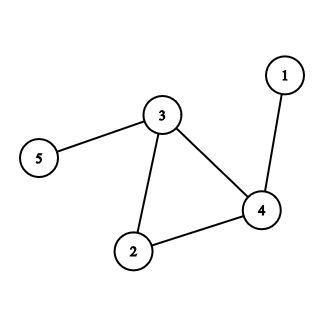
\includegraphics[width=0.5\textwidth]{unweighted_graph.png}
    \caption{Primer neusmerjenega grafa}
    \label{fig:mesh1}
\end{figure}

Zapis za graf na sliki je $G = (\{1, 2, 3, 4, 5\}, \{\{1, 4\}, \{4, 3\}, \{4, 2\}, \{3, 2\}, \{5, 3\}\})$

\subsubsection{Usmerjenost grafa}

Poznamo neusmerjene in usmerjene grafe. Za neusmerjen graf velja, da je povezava $v \in V$ množica moči dve, v kateri sta dve vozlišči. Za množice velja, da je $\{a, b\} = \{b, a\}$ (če velja, da je vozlišče a povezano z vozliščem b, je tudi vozlišče b povezano z vozliščem a). Pri usmerjenem grafu je povezava urejen par, velja, da je množica $E \subseteq (V \times V)$. Za urejene pare velja $(a, b) \neq (b, a)$ iz tega sklepamo, da povezava $a \rightarrow b$ ni enaka $b \rightarrow a$ oziroma ni nujno, da nasprotna povezava v grafu sploh obstaja.

\begin{figure}[H]
    \centering
    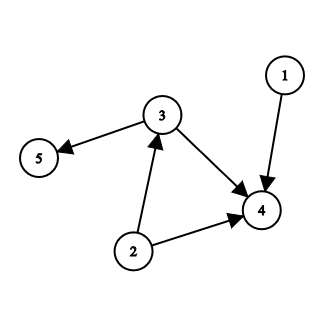
\includegraphics[width=0.5\textwidth]{directed_graph.png}
    \caption{Primer usmerjenega grafa}
    \label{fig:mesh1}
\end{figure}

Zapis za usmerjen graf na sliki je $G = (\{1, 2, 3, 4, 5\}, \{(1, 4), (3, 4), (2, 4), (2, 3), (3, 5) \})$

\subsubsection{Uteženost grafa}

Vsak graf je lahko utežen ali neutežen. Če je graf utežen, to pomeni, da lahko vsaki povezavi grafa določimo utež, vrednost ki ima lahko poljuben pomen, na primer razdaljo med dvema točkama, ceno postavitve ceste med dvema mestoma, moč kovalentne vezi med dvema atomoma itd. 

\subsubsection{Red in velikost}

Red grafa G definiramo kot moč množice $V(G)$, velikost grafa pa kot moč množice $E(G)$.

\subsubsection{Sosednost}

Sosednost je lastnost, definirana med dvema vozliščema neusmerjenega grafa, ki nam pove, da med točkami obstaja povezava. Matematično to zapišemo kot $a \sim b$.

\subsubsection{Stopnja vozlišča}

Vozlišču $v \in V(G)$ lahko določimo stopnjo $deg(v)$, za katero v neusmerjenem grafu velja, da je enaka številu vseh sosednjih vozlišč.
\\ \\
V usmerjenem grafu lahko vsakemu vozlišču določimo vhodno in izhodno stopnjo. \textbf{Vhodna stopnja} vozlišča usmerjenega grafa $deg^+(v)$ nam pove število predhodnikov tega vozlišča oziroma število povezav v grafu, ki začnejo na poljubnem vozlišču in končajo v tem vozlišču, \textbf{izhodna stopnja} $deg^-(v)$ pa število njegovih naslednjikov oziroma število povezav, ki začnejo v tem vozlišču.

\subsubsection{Oddaljenost}

Oddaljenost je definirana med dvema vozliščima grafa. Pri neuteženem grafu je oddaljenost število povezav, ki jih moramo prečkati, da iz prvega dosežemo drugo vozlišče. Pri uteženem grafu je oddaljenost seštevek vseh uteži povezav na poti od prve do druge točke. Ker lahko med dvema vozliščema obstaja več različno dolgih poti, nas po navadi zanima najmanjša oziroma največja oddaljenost. Za vozlišči, med katerima pot ne obstaja, definiramo oddaljenost med njima kot neskončno mnogo.

\subsubsection{Ekscentričnost vozlišča}

Ekscentričnost vozlišča je oddaljenost trenutnega vozlišča do najbolj oddaljenega vozlišča v grafu. \cite{eks}

\subsubsection{Gostota grafa}

Gostota grafa je lastnost grafa, ki nam pove razmerje med številom povezav grafa in maksimalnim številom povezav, ki jih graf z enakim številom vozlišč lahko ima.
\\ \\
Maksimalno število povezav za določen graf je:
\begin{gather*}
	\vert E \vert = \dfrac{\vert V \vert (\vert V \vert - 1)}{2}
\end{gather*}

(neusmerjen graf) in

\begin{gather*}
	\vert E \vert = \vert V \vert (\vert V \vert - 1)
\end{gather*}

(usmerjen graf).


\subsection{Povezan in nepovezan graf}

Graf je povezan, če obstaja pot med katerimakoli poljubnima vozliščema. Če graf ni povezan pravimo, da je ločen na komponente. Povezavi, ki bi, če bi jo odstranili, pomenila, da bi imel graf eno komponento več, rečemo \textbf{most}. \cite{studentka}


\subsection{Drevo}

Drevo je graf brez ciklov. Pri usmerjenih drevesih poznamo \textbf{navzven usmerjeno drevo} - vhodnja stopnja vseh razen enega vozlišča $deg^+(v) = 1$, vozlišču katerega stopnja je enaka 0 pravimo \textbf{koren drevesa}. Za \textbf{navznoter usmerjeno drevo} velja da je izhodnja stopnja kateregakoli vozlišča $deg^-(v) = 1$, izhodna stopnja korena pa je 0.

\subsection{Podgraf}

Graf K je podgraf grafa G, če velja da je $K_V \subseteq G_V$ in $K_E \subseteq G_E$. \cite{studentka}

\subsubsection{Vpeti podgraf}

Vpeti podgraf grafa G je graf K, za katerega velja $K_V = G_V$ in $K_E \subseteq G_E$. \cite{studentka}

\subsubsection{Najmanjše vpeto drevo}

Najmanjše vpeto drevo uteženega grafa je vpeti podgraf, ki je drevo in za katerega velja, da je vsota uteži vseh povezav minimalna možna. Graf ima lahko več minimalnih vpetih dreves. \cite{MST}

\subsection{Dvodelni graf}

Graf G je dvodelen, če obstaja porazdelitev množice $V(G)$ v dve podmnožici, tako da velja $V(G) = X \cup Y$ in da za vsako povezavo grafa velja, da je ena od krajiščnih točk povezave v množici $X$, druga pa v množici $Y$. Dvodelnost grafa lahko definiramo tudi tako, da je graf dvodelen, če je 2-obarvljiv (glej naslov k-obarvljivost). \cite{studentka}

\subsection{Polni graf}

Polni graf je graf, v katerem obstaja povezava med katerimakoli različnima vozliščema. Polni graf z $n$ vozlišči označimo z $K_n$. Gostota keteregakoli polnega grafa je 1. \cite{zapiski}

\subsubsection{Polni dvodelni graf}

Polni dvodelni graf $K_{m,n}$ je dvodelni graf, ločen na dve komponenti moči $m$ in $n$, pri katerem je vsako od m-tih vozlišč povezano z vsakim od n-tih. \cite{studentka}

\subsection{Minor}

Minor grafa G je graf M, do katerega pridemo, če na grafu G brišemo vozlišča, brišemo povezave ali krčimo povezave (zbrišemo povezavo med dvema vozliščema, nato pa obe vozlišči združimo v eno). \cite{planar}

\subsection{Ravninski graf}

Graf G je ravninski, če ga je mogoče narisati na ravnino, ne da bi se katerekoli od povezav sekale. Wagnerjev izrek pravi, da je graf planaren če in samo če kot minorja ne vsebuje grafa $K_5$ (polnega grafa 5 vozlišč) ali grafa $K_{3, 3}$ (polnega dvodelnega grafa šestih vozlišč). \cite{planar, studentka}

\begin{figure}[H]
    \centering
    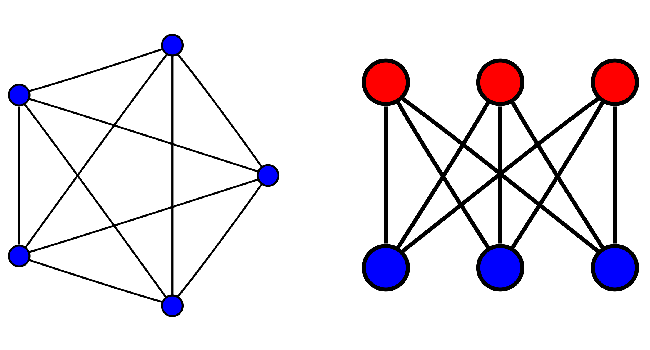
\includegraphics[width=0.5\textwidth]{k5_k33.png}
    \caption{Grafa $K_5$ in $K_{3, 3}$ \cite{planar}}
    \label{fig:mesh1}
\end{figure}


\subsection{Sprehod}

Na grafu lahko definiramo sprehod kot zaporedje povezav in točk grafa $v_0, e_0, v_1, e_1 ... v_k$, kjer je $e_i$ povezava med točkama $v_i$ in $v_{i-1}$. Dolžina sprehoda je definirana kot število povezav, ki smo jih na sprehodu prečkali.
\\ \\
\textbf{Enostaven sprehod} je sprehod, kjer se povezave v zaporedju ne ponovijo. \cite{studentka}

\subsubsection{Pot}

Pot je enostaven sprehod, kjer se tudi vozlišča ne ponavljajo. \cite{studentka}

\subsubsection{Obhod}

Obhod je sklenjen sprehod, velja $v_0 = v_k$. \cite{studentka}

\subsubsection{Cikel}

Cikel je pot, ki je obhod. \cite{studentka}

\subsubsection{Hamiltonov cikel}

Hamiltionov cikel je cikel, ki obišče vsako vozlišče na grafu. \cite{studentka}

\subsection{Barvanje grafa}

Barvanje grafa je preslikava $C(v) \rightarrow barva$, ki vsakemu elementu iz množice $G(V)$ priredi vrednost (barvo). Pri prirejanju barv mora veljati, da barvi katerihkoli sosednjih vozlišč ne smeta biti enaki. Poleg barvanja vozlišč poznamo tudi barvanje povezav in barvanje lic (samo za ravninske grafe). \cite{studentka, barvanjeWiki}

\subsubsection{K-obarvljivost}

K-obarvljivost je lastnost grafa G, ki nam pove, če obstaja preslikava $f: G(v) \rightarrow \{1, \dots, k\}$, oziroma če lahko graf G obarvamo s $k$ barvami. \cite{studentka, barvanjeWiki}

\subsubsection{Kromatično število grafa}

Kromatično število je lastnost grafa, označena z $\gamma(G)$, ki nam pove najmanjše število barv, s katerim je graf še obarvljiv. \cite{studentka, barvanjeWiki}

\section{Teoretične osnove NP-polnosti}


\subsection{Turingov stroj in deterministično reševanje problemov}

Turingov stroj je abstraktni računski model, ki ga je definiral angleški matematik Alan Turing. Stroj ima na voljo neomejeno dolg trak spominskih celic, po katerih se premika, nanje zapisuje in iz njih bere. Sposoben je izvajanja logičnih operacij in shranjevanja stanj. \textbf{Stanje} je navodilo, ki Turingovemu stroju narekuje, na kakšen načn naj se premika po traku, katere podatke naj bere in zapisuje nanj, ter na katero stanje naj se premakne po kočnanem izvajanju sledečega. Ko pride stroj do stanja, ki mu narekuje zaustavitev, pusti za sabo spremenjen trak z informacijami, ki predstavlja rešitev določenega problema.
\\ \\
Turingov stroj je osnova za \textbf{deterministično reševanje problemov} - reševanje, pri katerem definiramo točno določen algoritem, ki problem vedno reši na enak način in ki za enake vhodne podatke vedno vrne enak rezultat. Deterministično reševanje problemov zagotovi, da iz postopka izključimo vse človeške faktorje, kot so predstava in intuicija, in tako poskrbi, da lahko problem rešujemo z uporabo računalnika. \cite{TuringMachine, TuringVideo}

\subsection{Polinomska izračunljivost problema}

Polinomska izračunljivost je lastnost problema v teoriji izračunljivosti, ki nam pove, ali je določen problem možno deterministično rešiti v \textbf{polinomski časovni zahtevnosti} (tako, da bo funkcija, ki predstavlja časovno zahtevnost algoritma, polinom) z uporabo determinističnega Turingovega stroja. Vsi v algoritmi v poglavju Osnovni algoritmi so deterministični in imajo polinomsko časovno zahtevnost, kar pomeni, da so problemi, ki jih algoritmi rešijo, polinomsko izračunljivi.

\subsection{Problemi odločitev}

Problemi odločitev so problemi v obliki vprašanj, na katera lahko odgovorimo z da ali ne.

\subsection{NP problemi}

NP je oznaka, ki označuje vsak problem odločitve, ki je \textbf{polinomsko preverljiv} - to pomeni, da je možno rešitev mogoče preveriti v polinomski časovni zahtevnosti. \cite{np}

\subsection{P problemi}

P problem je vsak problem odločitve, ki je \textbf{polinomsko izračunljiv}. Vsak P problem je tudi NP problem - ker je že sam problem polinomsko rešljiv, lahko možno rešitev polinomsko preverimo preprosto tako, da jo izračunamo sami. \cite{p}

\subsection{NP težki probmemi}

NP težak problem je vsak problem, v katerega bi lahko v polinomskem času \textbf{reducirali} vsak NP problem. Redukcija v polinomskem času pomeni, da bi v primeru polinomske rešitve enega NP težkega problema lahko isti algoritem uporabili za polinomsko reševanje vseh ostalih NP problemov. Za NP težke probleme ne pozanmo polinomske rešitve, kar pomeni, da so algoritmi, ki jih uporabljamo za njihovo reševanje praktično neuporabni za vse razen najmanjših različic problemov, ki pa v praktičnem smislu nimajo posebnega pomena. \cite{nph}

\subsection{NP polni probmemi}

NP poln problem je problem, ki je hkrati NP težak (polinomsko nerešljiv) in NP (polinomsko preverljiv). \cite{npc}

\subsection{Hevristično reševanje problemov}

Probleme, katerih klasične metode reševanja so prepočasne, oziroma točne metode, ki zagotavlja najboljšo rešitev, sploh ne poznamo, rešujemo hevristično. Hevristično reševanje problema pomeni, da v reševanje vpeljemo različne predpostavke, ki niso nujno vedno resnične in tako reševanje pospešimo oziroma olajšamo. Rešitev, do katere smo prišli na tak način, ni nujno najboljša, vendar gre v marsikaterem primeru za dovolj dober približek, da je še vedno uporabna. Večina NP težkih problemov se v praksi rešuje hevristično. \cite{hevristika}

\subsection{Problem P vs. NP}

Vprašanje P vs. NP je eden od sedmih problemov tisočletne nagrade, ki jih je v letu 2000, skupaj z nagrado v višini milijon dolarjev za pravilno rešitev kateregakoli od njih, objavil Clayjev matematični inštitut. Problem sprašuje, ali dejstvo, da je problem polinomsko preverljiv (del množice NP) pomeni, da je tudi polinomsko rešljiv (del množice P). Problem za enkrat ostaja nerešen, njegova rešitev (v primeru, da bi se izkazalo da sta množici P in NP v resnici ena sama množica), pa bi pomenila preobrat v svetu računalništva, ki ga poznamo danes. Med probleme, ki bi jih v primeru takšnega odkritja lahko (učinkovito) reševali spadajo razni problemi povezani z iskanjem vzorcev, kot so izgradnja natančnih modelov za predvidevanje sprememb na finančnih trgih, analiza zlaganja proteinov v celici, sprejemanje optimalnih odločitev v različnih miselnih igrah (npr. šah, sudoku) in nazadnje faktorizacija velikih sestavljenih števil, kar bi podrlo temelje današnji enkripciji, ki jo na dnevni bazi za varno deljenje podatkov uporablja skoraj vsak izmed nas. \cite{pvnp, pvnpVideo, pvnpVpliv}

\begin{figure}[H]
    \centering
    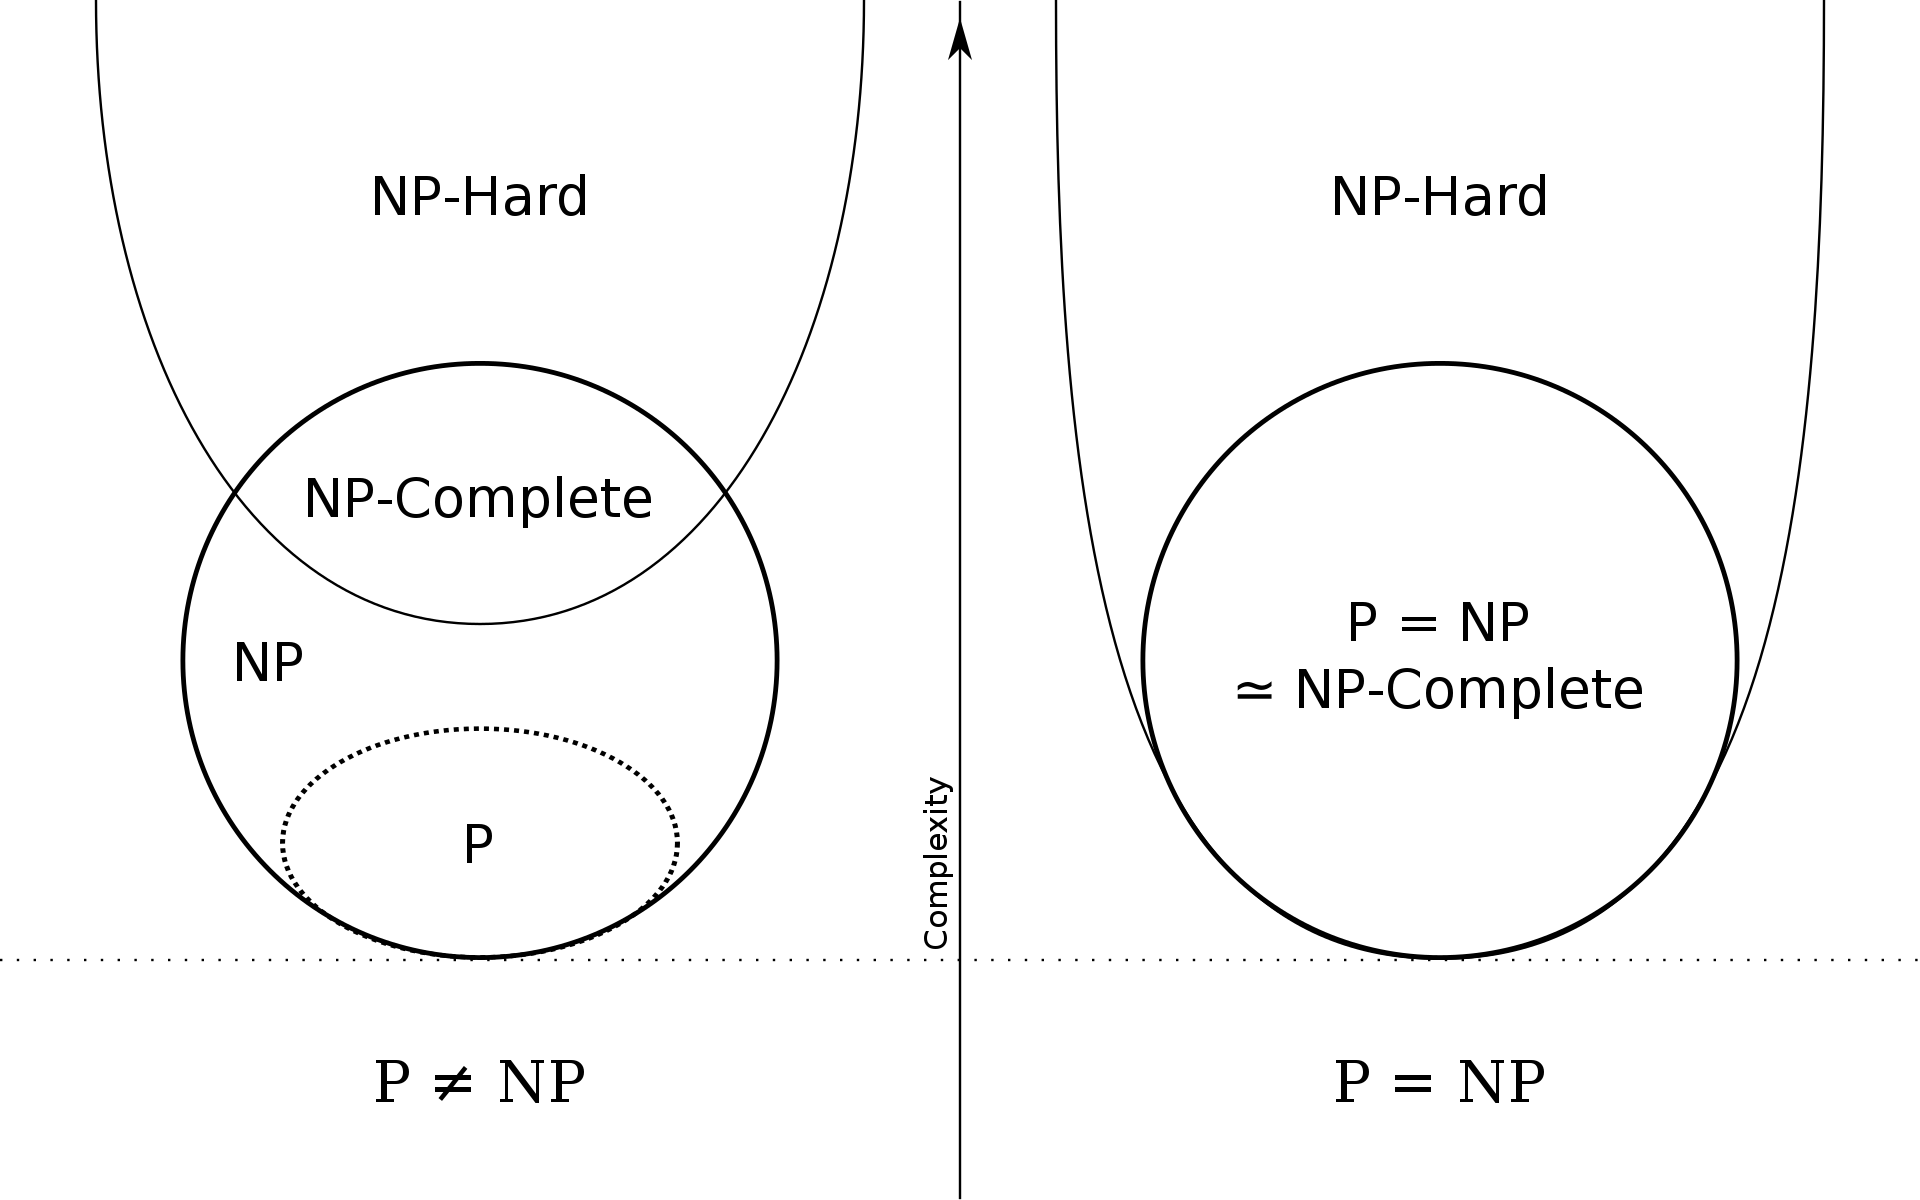
\includegraphics[width=0.5\textwidth]{P_vs_NP.png}
    \caption{Vizualni prikaz zgoraj omenjenih množic za obe teoriji \cite{pvnp}}
    \label{fig:mesh1}
\end{figure}


\section{Implementacija grafa}

Graf lahko v računalniku predstavimo na vrsto različnih načinov, kjer ima vsak način svoje prednosti in slabosti. Optimalen način implementacije je odvisen od gostote, uteženosti in usmerjenosti grafa, predvsem pa od tega, kaj želimo z grafom početi (ali pomembno hitro dodajanje in brisanje vozlišč, ali je pomembnejše hitrejše pregledovanje relacij med vozlišči). V tej raziskovalni nalogi sem se osredotočal predvsem na matriko sosednosti in seznam sosednosti, ki sta najpogostejša in najbolj generalna pristopa, vendar pa poznamo še vrsto drugih načinov, poleg tega pa lahko dodatno optimizacijo dosežemo tudi s kombiniranjem obeh pristopov.

\subsection{Matrika sosednosti}

Matrika sosednosti je eden najpogostejših pristopov k predstavitvi grafa. Osnovna ideja je, da za graf G določinmo matriko velikosti $n \times n$, kjer je $n$ red grafa G in z vsakim poljem matrike $a_{ij}$ predstavimo relacijo med i-tim in j-tim vozliščem v grafu. Če je graf neutežen lahko v matriko zapišemo 1 če povezava obstaja v nasprotnem primeru pa 0. V primeru uteženega grafa pa lahko lahko polje $a_{ij}$ predstavlja težo povezave med vozliščema $i$ in $j$. Če je graf, ki ga predstavljamo neusmerjen, bo matrika simetrična. Matrika sosednosti omogoča, da v časovni zahtevnosti $O(1)$ dobimo relacijo med dvema vozliščima, vendar pa je prostorsko precej neučinkovita z zahtevnostjo $O(n^{2})$, ne glede na število povezav v grafu, zato jo je pametno uporabiti na grafih z veliko gostoto.

\[
	\begin{bmatrix}
		0 & 0 & 0 & 1 & 0 \\
		0 & 0 & 1 & 1 & 0 \\
		0 & 0 & 0 & 1 & 1 \\
		0 & 0 & 0 & 0 & 0 \\
		0 & 0 & 0 & 0 & 0 \\
	\end{bmatrix}
\]

\thickspace

\noindent
Primer matrike sosednosti za usmerjen graf na sliki 2. Ker graf na sliki ni povezan preveč gosto, ima večina polj matrike vrednost 0, kar je prostorsko potratno.


\subsection{Seznam sosedov}

Seznam sosedov za graf G je seznam dolžine reda G, ki za vsako vozlišče grafa hrani vsa vozlišča, s katerimi je trenutno vozlišče povezano (v primeru uteženega grafa lahko poleg vozlišča hrani še težo povezave). Prednosti seznama sosedov so, da je njegova prostorska zahtevnost $O(V+E)$, prav tako omogoča hitro iteracijo čez vse sosede nekega vozlišča. Slabosti pa so počasnejše preverjanje, ali povezava med dvema točkama obstaja in počasno brisanje povezav - oboje $O(deg(v))$. Namesto seznama lahko v implementaciji uporabljamo tudi višje podatkovne strukture, na primer hash tabele, kar še dodatno pospeši delovanje.

\subsection{Eksplicitna predstavitev}

Eksplicitna predstavitev grafa je način implementacije, ki je najbližje matematični definiciji grafa. Zaradi grafične predstavitve grafa sem za lastni praktični izdelek uporabil ta pristop (glej poglavje Izdelava grafičnega vmesnika). V spominu namesto grafa hranimo dva seznama. Prvi seznam predstavlja vsa vozlišča (najpreprostje števila od $1$ do $n$, ali pa povsem nove objekte lastnega razreda), drugi seznam pa povezave (lahko preprosto seznami dolžine 2 oziroma 3 če je graf utežen ali objekti lastnega razreda, ki predstavlja povezavo). Eksplicitna predstavitev je načeloma počasnejša od zgornjih dveh implementacij - preverjanje obstoja povezave ima časovno zahtevnost $O(E)$, saj je potrebna iteracije čez vse sosede. Predosti eksplicitne predstavitve so hitro brisanje povezav v $O(1)$ in majhna prostorska zahtevnost, še posebej za neusmerjen graf $O(V + E)$.


\section{Izdelava grafičnega vmesnika}

Praktični izdelek te seminarske naloge je programiranje grafičnega vmesnika, ki bi uporabniku probližal delovanje nekaterih algoritmov na grafih s pomočjo vizualizacije. Vmesnik je napisan v programskem jeziku Python s pomočjo modula Pygame. Pygame je odprtokodni Pythonov modul, napisan v kombinaciji programskih jezikov C in Python, ki na osnovi knjižnice SDL uporabniku omogoča delo z grafiko in zvokom. Poleg Pygame sem v projektu uporabil tudi modul pygame\_gui, ki je prav tako odprtokodna knjižnica, ki vsebuje vnaprej pripravljene razrede za izgradnjo gumbov, menijev in obrazcev za vnos v modulu Pygame. \cite{Pygame, PyGui}
\\ \\
Koda, skupaj z navodili za uporabo grafičnega vmesnika, je na voljo na platformi Github na elektnonskem naslovu \textit{https://github.com/galgantar/graph\_theory}.


\subsection{Razred \textit{Gui}}

Razred $Gui$ v datoteki $gui.py$ je glavni razred, ki vsebuje vse potrebne podatke za prikazovanja okna (atribut $window$, dimenzije zaslona, font \dots), prikazovanja grafa (ki je med drugim eden od njegovih atributov), sledenje dogodkom in prikazovanja vseh elementov vmesnika. V poročilu naloge se bom osredotočal le na ključne dele objekta, ki so nujni za njegovo delovanje, celotna koda pa je na voljo na Github-u. Objekt v inicializacijiski funkciji poskrbi, da predpripravi vse svoje atrubute in vse podobjekte, iz katerih je zgrajen. Nato do prekinitve programa zaporedno kliče funkcijo \textit{Gui.refresh()}, ki nato poskrbi za osveževanje celotnega vmesnika. Funkcija \textit{Gui.refresh()} se torej pokliče 30-krat na sekundo (za časovne razmake med klici skrbi objekt $clock$) in preveri vse dogodke, ki so se zgodili do prejšnjega klica, ustrezno reagira na vnose miške in tipkovnice in na koncu z metodo \textit{Gui.draw\_items()} na novo nariše celoten grafični vmesnik in graf.
\\ \\
Vmesnik med drugim omogoča risanje svojega grafa, ki ga lahko uporabnik shrani za kasnejšo uporabo. Shranjevanje objektov v Pythonu omogoča standardna knjižnica pickle, ki vse podatke objekta shrani v posebno datoteko s pripono .pkl. Vse shranjene grafe lahko najdemo v mapi \textit{/saved\_graphs}. Shranjevanje in nalaganje grafov iz diska računalnika omogočata metodi \textit{Gui.save\_custom\_graph()} in \textit{Gui.load\_graph\_from\_a\_file()}.
\\ \\
Uporabnik lahko grafu, na vmesniku doda vozlišče, izbriše vozlišče, premika vozlišča, na novo obteži povezavo in poveže dve še nepovezani vozlišči. Vse to počne z uporabo miške in tipkovnice. Vnos iz teh dveh kanalov vmesnik sprejema s pomočjo metod \textit{Gui.handle\_mouse()} in \textit{Gui.handle\_keys()}.
\\ \\
Razred $Color$ v datoteki $color.py$ je namenjen predstavitvi barv in poleg RGB vrednosti \\ posameznih barv vsebuje funkcije, ki generirajo barve, uporabne pri vizualizaciji algoritmov.

\subsection{Razred \textit{Graph}}

Glavni atribut razreda $Gui$ je razred $Graph$. Gre za posebno implementacijo grafa, ki omogoča vmesniku shranjevanje še nekaterih, za klasične grafe nepotrebnih podatkov, ki so pomembni za vizuelno predstavitev grafa. Kot sem že omenil gre za eksplicitno predstavitev grafa, kjer namesto grafa hranimo dve množici, v prvi so vsa vozlišča in v drugi vse povezave med njimi. V progam smo dodali dva nova razreda Vozlišče ($Node$) in Povezava ($Edge$), kar dovoljuje, da poleg osnovnih podatkov o vsakem vozlišču in povezavi, hranimo še barvo, položaj in velikost.
\\ \\
Tako razred $Graph$ kot tudi $Node$ in $Edge$ imajo svoje metode, ki olajšajo implementacijo algoritmov na grafu. \textit{Graph.get\_edges\_from\_node(node)} je generator, ki omogoča iteracijo čez vse sosednje povezave nekega vozlišča, kljub temu, da so vsa vozlišča shranjena v množici. \textit{Graph.get\_edge(node1, node2)} vrne kazalec, če povezava med vozlišči obstaja in \\ \textit{Graph.are\_connected(node1, node2)} preveri prisotnost povezave. Graf z metodami omogoča tudi dodajanje in odstranjevanje povezav in vozlišč.
\\ \\
Vsaka povezava in vozlišče imata svojo metodo $draw()$, ki objekt nariše na zaslon in \textit{color\_element()}, ki objekt pobarva. Za razrede so implemetirane tudi tako imenovane magične metode \\ ($\_\_hash\_\_$, $\_\_repr\_\_$, $\_\_eq\_\_$ \dots), ki objektom omogočajo še višji nivo abstrakcije in spajanje z osnovnimi Pythonovimi podatkovnimi strukturami (npr. hash tabela - $set$) in operatorji ($<$, $==$, $[]$).

\begin{figure}[H]
    \centering
    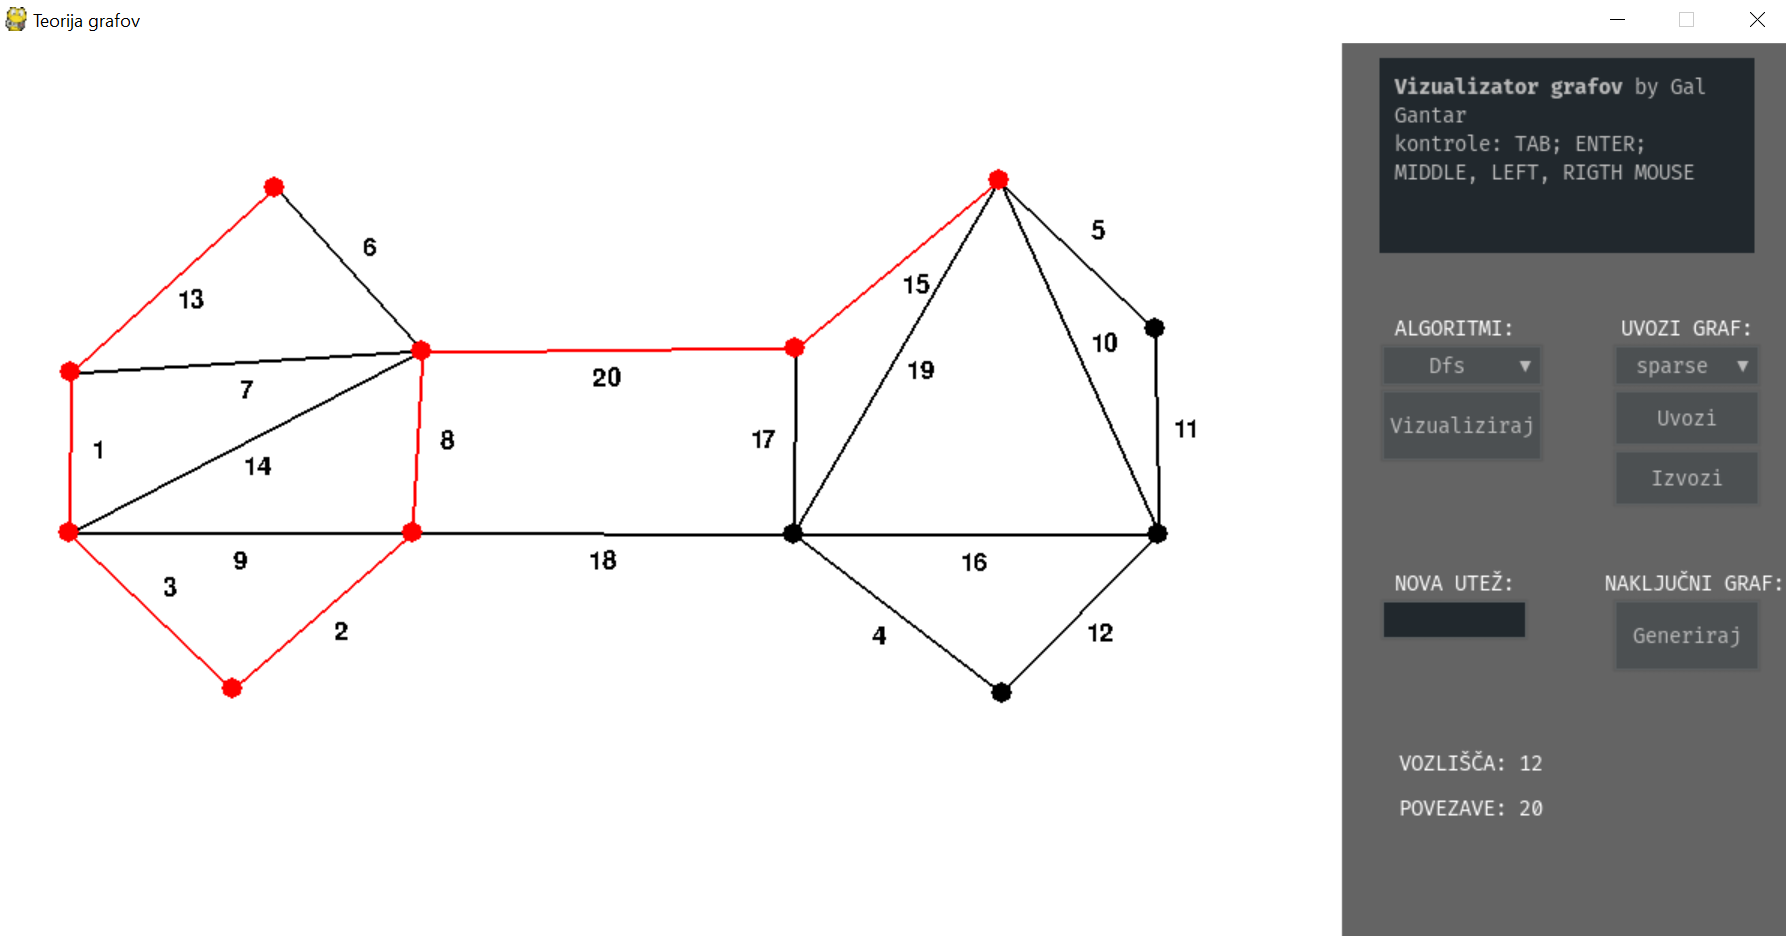
\includegraphics[width=1\textwidth]{gui_example.png}
    \caption{Grafični vmesnik}
    \label{fig:mesh1}
\end{figure}

\section{Osnovni algoritmi}

Kot del raziskovalne naloge sem napisal program, ki vizualizira delovanje nekaterih osnovnih algoritmov na neusmerjenem uteženem grafu. Vsi algoritmi so implementirani v datoteki $algorithms.py$, vendar sem v nalogo vključil krajše verzije istih algoritmov, ki se ne rišejo na zaslon, saj je koda tako krajša in veliko bolj pregledna.

\subsection{Preiskovanje v globino}

Preiskovanje v globino (ang. $DFS$) je najpreprostejši način prečkanja grafa. Časovna zahtevnost algoritma je $O(V + E)$ ob rekurzivni implementaciji pa ima v najslabšem primeru prostorsko zahtevnost $O(V)$. Preiskovanje v globino lahko uporabimo za iteracijo čez vsa vozlišča, dosegljive iz poljubnega vozlišča, kot je prikazano v spodnjem primeru. Funkcija kot parametre sprejme objekt razreda $Graph$ in objekt razreda $Node$, ki predstavlja vozlišče iz katerega bi radi iskali dosegljiva vozlišča. Na začetku vsakega rekurzivnega klica z $yield$ iz funkcije "podamo" vozlišče in ga dodamo v seznam $visited$, nato pa poiščemo vsa sosednja vozlišča, ki jih še nismo obiskali in za vsakega naredimo rekurzivni klic (6-8). Seznam $visited$ skozi rekurzijo ostaja enak za vse nadaljne klice, saj si funkcije kot parametre podajajo le kazalec do seznama in ne naredijo nove kopije za vsak klic. \cite{dfs}

\begin{lstlisting}[language=Python, caption=Presikovanje v globino]
def dfs(G, current, visited=None):
	if visited is None: visited=set()
    yield e.second_node    
    visited.add(current)

    for e in G.get_edges_from_node(current):
        if e.second_node not in visited:
            dfs(G, e.second_node, visited)

    
\end{lstlisting}

\subsection{Preiskovanje v širino}

Preiskovanje v širino (ang. $BFS$) je prav tako kot preiskovanje v globino način preiskovanja grafa z začetkom v poljubnem vozlišču. Časovna zahtevnost algoritma je prav $O(V + E)$, prostorska zahtevnost pa je v najslabšem primeru $O(V)$. Preiskovanje v širino lahko uporabljamo za iskanje najkrajše poti med dvema točkama, ob predpostavki da so vse povezave enako utežene, oziroma za računanje oddaljenosti (najmanjšega števila povezav) med dvema točkama. Prav tako lahko algoritem uporabimo za določanje ekscentričnosti vozlišča. Spodaj je primer uporabe preiskovanja v širino za določanja minimalne oddaljenosti dveh vozlišč.
\\ \\
Funkcija kot parametre sprejme graf in dva objekta razreda $Node$, ki predstavljata izhodiščno in končno vozlišče. Lokalna spremenljivka Q predstavlja vrsto (uvoženo iz standardnega Pythonovega modula collections), spremenljivka $visited$ predstavlja množico že obiskanih točk. Na začetku v vrsto dodamo izhodiščno vozlišče skupaj z razdaljo (razdalja od vozlišča do samega sebe je 0). Dokler vrsta Q ni prazna iz začetka vrste vzamemo vozlišče in njegovo oddaljenost od izhodišča, preverimo, ali gre za iskano vozlišče in če gre, vrnemo razdaljo (7,8). V nasprotnem primeru pa na konec vrste dodamo vsa trenutnemu vozlišču sosednja vozlišča, ki jih še nismo obiskali skupaj z razdaljo, povećano za 1, ter vozlišča dodamo v množico $visited$ (10-13). Če se vrsta Q izprazni, preden najdemo iskano vozlišče, to pomeni, da vozlišče iz izhodiščnega vozlišča ni dostopno. V tem primeru je oddaljenost neskončna (15). \cite{bfs}

\begin{lstlisting}[language=Python, caption=Presikovanje v širino]
def bfs(G, start, end):
    visited = set()
    Q = collections.deque()
    Q.append((0, start))
    while Q:
        dist, N = Q.popleft()		
        if N == end:
	        return dist        
        
        for e in G.get_edges_from_node(N):
            if e.end_node not in visited:            
                Q.append((dist + 1, e.end_node)
                visited.add(e.end_node)
    
    return float("inf")
    
\end{lstlisting}

\subsection{Primov algoritem}

Primov algoritem je algoritem, namenjen iskanju najmanjšega vpetega drevesa v grafu. Gre za tako imenovani \textbf{požrešni algoritem}, kar pomeni, da do rešitve večjegra problema pride tako, da večkrat zaporedno izbere opcijo, ki je v danem trenutku optimalna rešitev preprostejšega problema. Algoritem začne v poljubnem vozlišču in si shrani vse povezave, ki vključujejo to vozlišče. Nato izmed vseh povezav izbere najcenejšo in nato prejšnjim shranjenim povezavam doda še vse povezave, ki vodijo iz končne točke izbrane povezave. Postopek ponavlja, dokler ni obiskal vseh vozlišč v grafu. Vse povezave, ki jih je na poti izbral predstavljajo najmanjše vpeto drevo.
\\ \\
Funkcija sprejme graf ter $visited$ in $MST$ (ang. minimum spanning tree) nastavi na prazni množici. Nato spremenljivko $first$ nastavi na naključno vozlišče (to naredi s pomočjo iteratorja čez množico $nodes$ v grafu). Prvo vozlišče doda v $visited$, nato pa zgradi minimalno kopico (prioritetno vrsto) iz vseh povezav, ki vsebujejo vozlišče $first$ (5). Nato v zanki jemlje povezave iz kopice ter za vsako povezavo preveri, ali trenutno vozlišče povezuje s še neobiskanim vozliščem (10). Ko najde tako povezavo, jo doda minimalnemu vpetemu drevesu (prioritetna vrsta skrbi, da bodo najprej prišle na vrsto najcenejše povezave), vozlišče doda obiskanim vozliščem in nato vse povezave, ki vodijo iz tega vozlišča doda v vrsto (11-14). Postopek ponavlja, dokler niso bila obiskana vsa vozlišča. \cite{prims}

\begin{lstlisting}[language=Python, caption=Primov algoritem]
def prims(G):
    visited, MST = set(), set()
    first = next(iter(G.nodes))
    visited.add(first)
    all_edges = list(G.get_edges_from_node(first))
    heapq.heapify(all_edges)
    
    while len(visited) < G.order:
       e = heapq.heappop(all_edges)
       if e.first_node not in visited and e.second_node not in visited:
           MST.add(e)
           visited.add(e.second_node)
           for edge in G.get_edges_from_node(e.second_node):
               heapq.heappush(all_edges, edge)
    return MST
        
    
\end{lstlisting}


\subsection{Boruvkov algoritem}

Boruvkov algoritem prav tako najde najmanjše vpeto drevo v grafu. Enako kot pri Primovem algoritmu gre za požrešni algoritem. Algoritem se problema loti tako, da vsakemu vozlišču poišče najcenejšo povezavo, ki izhaja iz njega. Tako formira tako imenovan \textbf{gozd} - množico poddreves grafa (v prvi iteraciji so ima vsako drevo le eno vozlišče). Nato vsakemu drevesu poišče najcenejšo povezavo in tako drevo združi z enim od sosednjih dreves. To ponavlja, dokler v gozdu ne ostane le eno drevo - to predstavlja eno od najmanjših vpetih dreves grafa. Ena od prednosti Boruvkovega algoritma je, da ga lahko enostavno preobrazimo tako, da išče vpeta drevesa v komponentah nepovezanih grafov.
\\ \\
Funkcija v začetku seznam forest napolne z  $\vert V \vert $ seznami dolžine 1, vsak od katerih vsebuje eno vozlišče (2). Minimalno vpeto drevo ($MST$) nastavi na prazno množico. Nato v zanki vsakemu vozlišču v grafu z metodo $make\_mark()$ doda oznako komponente, kateri vozlišče pripada (6-8). Seznam $cheapest$ predstavlja najcenejše povezave za vsako posamezno komponento (10). Z zanko nato iteriramo čez vse povezave v grafu in poiščemo najcenejše povezave , ki povezujejo dve različni komponenti gozda (12-17). Najcenejše povezave med komponentami nato dodamo minimalnemu vpetemu drevesu, komponente, ki jih povezujejo pa združimo (20-24). Ko ima gozd le eno komponento izstopimo iz zanke in vrnemo najmanjše vpreto drevo (27). \cite{boruvkas}


\begin{lstlisting}[language=Python, caption=Boruvkov algoritem]
def boruvkas(G):
    forest = [{node} for node in G.nodes]
    MST = set()
    
    while len(forest) > 1:
        for i, component in enumerate(forest):
            for node in component:
                node.make_mark(i)
        
        cheapest = [None for _ in range(len(forest))]
        
        for e in G.edges:
            if e.first_node.mark != e.second_node.mark:
                if not cheapest[e.first_node.mark] or e < cheapest[e.first_node.mark]:
                    cheapest[e.first_node.mark] = e
                if not cheapest[e.second_node.mark] or e < cheapest[e.second_node.mark]:
                    cheapest[e.second_node.mark] = e
        
        new_forest = []
        for e in set(filter(None, cheapest)):
            MST.add(e)            
            C = forest[e.first_node.mark]
            C.extend(forest[e.second_node.mark]          
            new_forest.append(C)
            
        forest = new_forest
    return MST

\end{lstlisting}

\section{NP polni problemi na grafu}

NP polni problemi nastopajo v mnogo različnih oblikah. V tej raziskovalni nalogi bom opisal dva NP polna problema, ki ju lahko predstavimo s pomočjo grafa. Oba problema sta implementirana v grafičnem vmesniku, v nalogi pa sta vključeni skrajšani verziji, ki se ne rišeta na zaslon.

\subsection{Problem trgovskega potnika}

Problem trgovskega potnika je NP težak problem, ki sprašuje, kako dolga je najkrajša pot, ki se začne in konča v istem mestu in na poti obišče vsa ostala mesta v določeni množici mest. Problem je sam po sebi NP težak (ni problem odločitve, zato ga ni mogoče preveriti), vendar obstaja verzija problema, ki namesto iskanja najkrajše poti sprašuje, ali obstaja pot na grafu, ki je krajša od neke dolžine, ta verzija pa je NP polna (če že imamo pot, lahko preprosto s sledenjem tej poti preverimo, ali je seštevek vseh povezav na njej manjši od dane vrednosti).
\\ \\
Če problem predstavimo z grafom, vsakemu mestu dodelimo vozlišče, ter ga povežemo z vsemi ostalimi mesti v grafu tako, da utež povezave predstavlja razdaljo med mestoma. Nato želimo na tem grafu najti Hamiltonov cikel (želimo obiskati vsa vozlišča na grafu, brez ponavljanja vozlišč), katerega vsota vseh povezav bo najmanjša možna.
\\ \\
Za optimizacijo nimamo posebnega algoritma, zato moramo za iskanje najboljše rešitve preprosto preveriti vse možnosti (uporabiti preiskovanje s silo ang. brute force approach) in izmed njih izbrati najmanjšo. To lahko dosežemo z uporabo rekurzije - problem kako dolga je najkrajša pot, ki od trenutne točke obišče vse podane točke, lahko predstavimo kot minimum vseh poti, ki obiščejo vse točke razen ene od sosed te točke + teža povezave do sosede.
\\ \\
Funkcija sprejme graf G, začetno (in hkrati končno) vozlišče, trenutno vozlišče (v prvem klicu enako končnemu) in množico $remaining$, ki predstavlja vsa vozlišča, ki jih je še treba obiskati (pri prvem klicu so v množici vsa vozlišča grafa). Iz množice $remaining$ odstranimo trenutno vozlišče in nato, če je množica prazna, (kar pomeni, da smo obiskali vsako vozlišče in bi morali biti eno povezavo oddaljeni od konca poti) preveri, če v grafu obstaja povezava od vozlišča do konca in vrne njeno utež. Če povezava ne obstaja, vrnemo neskončno, saj ta pot ni veljavna (5-7). Spremenljivka $cost$ predstavlja najmanjšo vrednost poti, ki jo lahko opravimo, če pot začnemo v tem vozlišču in na poti obiščemo vsa vozlišča v množici $remaining$. V zanki nato za vsako od preostalih vozlišč poiščemo pot do vseh sosednjih vozlišč, ki so v množici $remaining$ (če nobeno tako vozlišče ne obstaja vrnemo začetno vrednost $cost$ - neskončno) in nato rekurzivno kličemo funkcijo z vsakim od sosednjih vozlišč ter vrnemo najmanjšo od teh vrednosti (11-18). \cite{TSP}


\begin{lstlisting}[language=Python, caption=Problem trgovskega potnika]
def TSP(G, start, curr, remaining):
    remaining.remove(curr)
    
    if not remaining:
        final = G.get_edge(start, curr)
        if final is None:
            return float("inf")
        return final.weight
    
    cost = float("inf")
    for node in remaining:
        e = G.get_edge(current, node)
        if e is None:
            continue
        
        cost = min(cost, e.weight + TSP(G, start, node, remaining))
        
    return cost

\end{lstlisting}

\subsection{Barvanje grafov in kromatično število}

Barvanje grafov z najmanjšim možnim številom barv (določanje kromatičnega števila grafa) je še en NP težak problem. Če problem preobrazimo tako, da nas zanima, ali je graf mogoče obarvati z $k$ barvami, tako kot pri primeru trgovskega potnika dobimo NP poln problem. Ker polinomska rešitev ne obstaja, lahko problem rešimo le z uporabo sile. Kljub temu, da polinomska rešitev ne obstaja, lahko zmanjšamo čas delovanja algoritma tako, da uporabimo backtracking oziroma, da namesto pregledovanja vseh možnih $k^n$ obarvanj nekega grafa sproti izločamo tiste, za katere že vemo, da niso veljavne. Kljub tej optimizaciji pa časovna zahtevnost v najslabšem primeru ostaja eksponentna.
\\ \\
Funkcija za določanje kromatičnega števila preprosto povečuje število barv, dokler graf ni obarvljiv. Funkcija za preverjanje obarvljivosti grafa z $n$ barvami, sprejme kot argumente graf G, množico vseh vozlišč, ki jih je treba obarvati, in število barv. Najprej pogledamo, če je množica vozlišč prazna, saj je graf z nič vozlišči mogoče obarvati z poljubno majhnim številom barv. Nato vsakemu vozlišču v množici priredimo vsako izmed možnih barv (12, 13) in nato s sosedami tega vozlišča preverimo, ali je taka razporeditev barv veljavna (14-16). Če neveljavnost ni najdena (v Pythonu se $else$ po $for$ zanki izvede, če nikjer v zanki nismo poklicali $break$), obarvamo vozlišče in nato z rekurzivnim klicom preverimo, ali obstaja kakršnokoli veljavno obarvanje preostalih vozlišč (15). Če veljavno obarvanje obstaja, vrnemo $True$, v nasprotnem primeru pa nadaljujemo s prirejanjem barv v zanki. Če veljavno obarvanje ni bilo najdeno vrnemo $False$. \cite{coloring}


\begin{lstlisting}[language=Python, caption=Določanje kromatičnega števila grafa]
def chromatic_number(G):
    k = 1    
    while not n_colourable(G, G.nodes.copy(), n):
        k += 1
    return k
    
    
def n_colourable(G, nodes, n):
    if not nodes:
        return True
    
    for node in nodes:
        for color in range(n):
            for edge in G.get_edges_from_node(node):
                if e.second_node.color == color:
                    break
            else:
                node.color = c
                if n_colourable(G, nodes - {node}, n):
                    return True
    return False

\end{lstlisting}

\section{Uporaba teorije grafov}

Računalniško ali cestno omrežje lahko predstavimo kot graf. Z iskanjem mostov na grafu lahko na omrežju iščemo šibkosti (na primer iskanje ceste na cestnem omrežju, ki bi, v primeru zaprtja, preprečila prehod iz enega mesta v drugo). Iskanje najmanjšega vpetega drevesa nam lahko pomaga poiskati nepotrebne povezave v omrežju (ugotavljanje, katere povezave med strežniki lahko odstranimo, da bi z minimalnimi stroški vzdrževanja omrežje še vedno omogočalo prenos podatkov vsem strežnikom). Najmanjše vpeto drevo lahko uporabimo za ugotavljanje, kakšna je najbolj optimalna izgradnja električnega omrežja med hišami, tako da je vsaka hiša priključena na omrežje. Iskanje najkrajše poti med dvema vozliščima v omrežju se uporablja v navigacijskih napravah v avtomobilih. 
\\ \\
Tudi socialna omrežja so v računalniškem smislu ogromni grafi uporabnikov, ki so med seboj povezani s prijateljstvi. Iskalniki kot so Google in Bing spletne strani vrednotijo s pomočjo grajenja usmerjenih grafov, kjer vozlišča predstavljajo spletne strani, povezave med njimi pa povezave, preko katerih lahko prehajamo med njimi. V nadaljevanju bo uporabnost teorije grafov prikazana še na praktičnih problemih.

\subsection{Načrtovanje poti}

Načrtovanje poti je eden od primerov, kjer si lahko pomagamo s teorijo grafov. Recimo, da se odpravljamo na potovanje z avtomobilom in si želimo na potovanju ogledati 5 različnih mest, pri tem pa za pot porabiti kar se da malo časa. Vrstni red obiska mest ni pomemben. Problem predstavimo z grafom tako, da vsakemu mestu pripišemo vozlišče, nato pa vsak par različnih mest povežemo z neusmerjeno obteženo povezavo, katere utež predstavlja čas potovanja iz enega mesta v drugo.

\begin{center}

\begin{tabular}{ c | c c c c c }
	
	 & $M_1$ & $M_2$ & $M_3$ & $M_4$ & $M_5$ \\ 
	\hline 
 	$M_1$ & $\times$ & 9 & 10 & 4 & 14 \\
 	$M_2$ & 9 & $\times$ & 10 & 12 & 10\\
 	$M_3$ & 10 & 10 & $\times$ & 10 & 7 \\
 	$M_4$ & 4 & 12 & 10 & $\times$ & 8\\
 	$M_5$ & 14 & 10 & 7 & 8 & $\times$ \\

\end{tabular}

\end{center}

\begin{center}
\null
\thinspace
Tabela prikazuje ure potovanja med posameznimi mesti
\end{center}

\noindent Nato na grafu poženemo algoritem za rešitev problema trgovskega potnika, ki nam izračuna načrt potovanja tako, da bo čas potovanja minimalen možen. Problem lahko rešimo z uporabo grafičnega vmesnika, graf za ta problem lahko uvozimo v program, nahaja se pod imenom "mesta".

\begin{figure}[H]
    \centering
    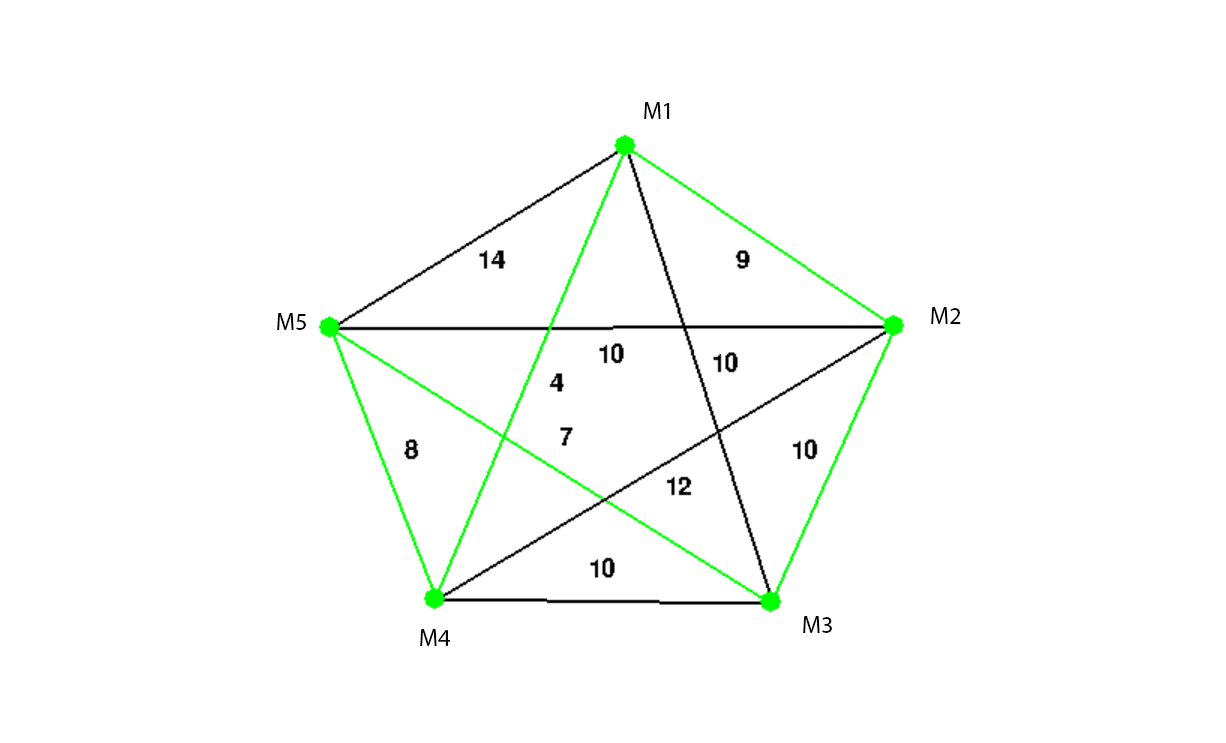
\includegraphics[width=0.8\textwidth]{TSP.png}
    \caption{Problem potovanja rešen z uporabo grafičnega vmesnika}
    \label{fig:mesh1}
\end{figure}


\subsection{Barvanje zemljevida}

Še en primer praktične uporabe grafov je barvanje zemljevida. Recimo da želimo pobarvati zemljevid držav tako, da nobeni sosednji državi ne bosta enake barve. To storimo tako, da vsako državo predstavimo kot vozlišče in jo nato z neusmerjeno povezavo povežemo z vsemi sosednjimi državami. Na grafu poženemo algoritem za barvanje grafa in s tem določimo barvo vsake države. Algoritem poskrbi, da bomo za barvanje porabili minimalno možno število barv. Tudi ta primer lahko v grafičnem vmesniku uvozimo pod imenom "aus".

\begin{figure}[H]
    \centering
    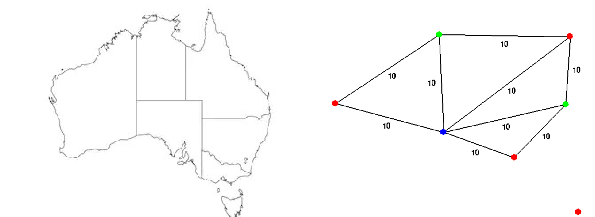
\includegraphics[width=0.8\textwidth]{australia.png}
    \caption{Barvanje zemljevida z uporabo grafičnega vmesnika \cite{ausIMG}}
    \label{fig:mesh1}
\end{figure}

\newpage
\section{Zaključek}

Cilj naloge je bil predstaviti grafe kot matematično strukturo, implementirati graf in izdelati grafični vmesnik, ki uporabnikom omogoča lažje razumevanje nekaterih algoritmov na grafih. Razumevanje teorije grafov postaja vse bolj uporabno znanje, saj so grafi z razvojem računalništva vstopili v naše vsakdanje življenje, ne da bi se tega sploh zavedali. Poleg tega, da jih uporabljamo v matematiki, od koder izvirajo, jih lahko najdemo v kemijskem, fizikalnem, biološkem in celo sociološkem raziskovanju. So sestavni del mnogih tehnologij, brez katerih bi si življenje danes težko predstavljali. Grafi nam odpirajo nov pogled na nekatere strukture okrog nas in omogočajo, da te strukture matematično predstavimo in analiziramo. Vsesplošna uporabnost grafov, je dokaz, da za matematične strukture ni nujno takoj očitno, zakaj so uporabne, ampak se njihova uporabna vrednost pokaže šele kasneje. To odpira možnost, da smo marsikatero prihodnje odkritje v svetu znanosti že analizirali, treba ga je le še pravilno interpretirati in mu pripisati pravi pomen.

\newpage
% Viri
\renewcommand{\refname}{Literatura}

\begin{thebibliography}{9}
	
	\bibitem{zapiski}
	\begin{flushleft} 
	 Matija Polajnar, Zapiski iz teorije grafov, 16.03.2006, 
	\href{https://www.fmf.uni-lj.si/~skreko/Pouk/ds2/Zapiski/Polajnar-DS2-1.pdf}{\textit{https://www.fmf.uni-lj.si/~skreko/Pouk/ds2/Zapiski/Polajnar-DS2-1.pdf}}. (citirano 6.2.2020)
	\end{flushleft}	
	
	\bibitem{psevdo}
	\begin{flushleft}
	Sodelavci Wikipedije, Multigraf, 11.7.2016, \textit{https://sl.wikipedia.org/wiki/Multigraf} (citirano 6.2.2020)
	\end{flushleft}
	
	\bibitem{studentka}
	\begin{flushleft}
	Ana Oblak, Teorija grafov, 16.12.2007, 
	\textit{http://www.educa.fmf.uni-lj.si/izodel/sola/2006/ura/oblak/html/Uvod.html} (citirano 6.2.2020)	
	\end{flushleft}
	
	\bibitem{eks}
	\begin{flushleft}
	Katja Kotnik, K-GEODOMINANTNE MNOŽICE V GRAFIH IN SORODNI KONCEPTI, 2016, strani 1-6
	\textit{https://core.ac.uk/download/pdf/67604584.pdf} (citirano 8.2.2020)
	\end{flushleft}	
	
	\bibitem{MST}
	\begin{flushleft}
	Minimalno vpeto drevo, 2.6.2007, 
	\textit{http://wiki.fmf.uni-lj.si/wiki/Minimalno\_vpeto\_drevo} (citirano 8.2.2020)
	\end{flushleft}
	
	\bibitem{planar}
	\begin{flushleft}
	Sodelavci Wikipedije, Planarni graf, 22.2.2020, 
	\textit{https://en.wikipedia.org/wiki/Planar\_graph} (citirano 8.2.2020)
	\end{flushleft}
	
	\bibitem{barvanjeWiki}
	\begin{flushleft}
	Sodelavci Wikipedije, Barvanje grafov, 7.2.2020, 
	\textit{https://en.wikipedia.org/wiki/Graph\_coloring} (citirano 8.2.2020)
	\end{flushleft}	
	
	\bibitem{TuringMachine}
	\begin{flushleft}
	Sodelavci Wikipedije, Turingov stroj, 8.1.2020, 
	\textit{https://en.wikipedia.org/wiki/Turing\_machine} (citirano 12.2.2020)
	\end{flushleft}	

	\bibitem{TuringVideo}
	\begin{flushleft}
    Youtube kanal Computerphile, Turingov stroj, 29.8.2014, 
	\textit{https://www.youtube.com/watch?v=dNRDvLACg5Q} (citirano 12.2.2020)
	\end{flushleft}
	
	\bibitem{np}
	\begin{flushleft}
	Sodelavci Wikipedije, NP kompleksnost, 2.2.2020, 
	\textit{https://en.wikipedia.org/wiki/NP\_(complexity)}	(citirano 14.2.2020)
	\end{flushleft}
		
	\bibitem{p}
	\begin{flushleft}
	Sodelavci Wikipedije, P kompleksnost, 9.11.2019, 
	\textit{https://en.wikipedia.org/wiki/P\_(complexity)} (citirano 14.2.2020)
	\end{flushleft}
		
	\bibitem{nph}
	\begin{flushleft}
	Sodelavci Wikipedije, NP težkost, 12.12.2019, 
	\textit{https://en.wikipedia.org/wiki/NP-hardness} (citirano 14.2.2020)
	\end{flushleft}
		
	\bibitem{npc}
	\begin{flushleft}	
	Sodelavci Wikipedije, NP popolnos, 18.12.2019, 
	\textit{https://en.wikipedia.org/wiki/NP-completeness} (citirano 14.2.2020)
	\end{flushleft}
	
	\bibitem{hevristika}
	\begin{flushleft}	
	Hevristični pristopi k reševanju problemov, 5.2.2018, 
	\textit{https://www.101computing.net/heuristic-approaches-to-problem-solving/} (citirano 22.2.2020)
	\end{flushleft}
		
	\bibitem{pvnp}
	\begin{flushleft}
	Sodelavci Wikipedije, P vs. NP problem, 12.1.2020, 
	\textit{https://en.wikipedia.org/wiki/P\_versus\_NP\_problem}(citirano 1.2.2020)
	\end{flushleft}
		
	\bibitem{pvnpVideo}
	\begin{flushleft}	
	Youtube kanal hackerdashery, P vs. NP, 26.8.2020, 
	\textit{https://www.youtube.com/watch?v=YX40hbAHx3s} (citirano 1.2.2020)
	\end{flushleft}
	
	\bibitem{pvnpVpliv}
	\begin{flushleft}
	John Pavlus, Kaj pomeni P vs. NP za nas?, 19.8.2010, 
	\textit{https://www.technologyreview.com/s/420290/what-does-p-vs-np-mean-for-the-rest-of-us/} (citirano 5.2.2020)
	\end{flushleft}
	
	\bibitem{Pygame}
	\begin{flushleft}
	Knjižnica Pygame, 
	\textit{https://www.pygame.org/wiki/about} (citirano 28.2.2020)
	\end{flushleft}
	
	\bibitem{PyGui}
	\begin{flushleft}	
	Repozitorij knjižnice pygame\_gui, 
	\textit{https://github.com/MyreMylar/pygame\_gui} (citirano 28.2.2020)
	\end{flushleft}
	
	\bibitem{dfs}
	\begin{flushleft}	
	Sodelavci spletne strani Geeks for geeks, Implementacija algoritma DFS, 
	\textit{https://en.wikipedia.org/wiki/Depth-first\_search} (citirano 10.12.2019)
	\end{flushleft}
	
	\bibitem{bfs}
	\begin{flushleft}	
	Sodelavci Wikipedije, Implementacija algoritma BFS, 
	\textit{https://en.wikipedia.org/wiki/Breadth-first\_search} (citirano 15.12.2019)
	\end{flushleft}
	
	\bibitem{prims}
	\begin{flushleft}	
	Sodelavci spletne strani Geeks for geeks, Implementacia Primovega algoritma, 
	\textit{https://www.geeksforgeeks.org/prims-minimum-spanning-tree-mst-greedy-algo-5/} (citirano 23.12.2019)
	\end{flushleft}	
	
	\bibitem{boruvkas}
	\begin{flushleft}	
	Sodelavci spletne strani Geeks for geeks, Implementacija Boruvkovega algoritma, \textit{https://www.geeksforgeeks.org/boruvkas-algorithm-greedy-algo-9/} (citirano 20.11.2019)
	\end{flushleft}	
	
	\bibitem{TSP}
	\begin{flushleft}	
	Youtube kanal Abdul Bari, Razlaga problema potujočega potnika, 22.2.2018, \textit{https://www.youtube.com/watch?v=XaXsJJh-Q5Y} (citirano 17.2.2020)
	\end{flushleft}	
	
	\bibitem{coloring}
	\begin{flushleft}	
	Sodelavci spletne strani Geeks for geeks, Implementacija barvanja grafa, \textit{https://www.geeksforgeeks.org/m-coloring-problem-backtracking-5/} (citirano 17.2.2020)
	\end{flushleft}	
	
	\bibitem{ausIMG}
	\begin{flushleft}
	Zemljevid Avstralije, \textit{https://fr.dreamstime.com/carte-l-australie-image114364535} (uporabljeno 29.2.2020)
	\end{flushleft}

\end{thebibliography}

\end{document}
